\documentclass[12pt, letterpaper, twoside]{article}
\usepackage[utf8]{inputenc}
\usepackage[english,russian]{babel}
\usepackage{tikz}  
\usetikzlibrary{graphs}
\usepackage{amsmath}
\DeclareMathOperator*{\argmin}{argmin} % no space, limits underneath in displays
\graphicspath{ {./} }
\usepackage{listings}


\title{First document}
\author{Serhy Makarenko \thanks{funded by the ShareLaTeX team}}
\date{December 2018}

\begin{document}
	
\begin{titlepage}
	\begin{center}
		\large



		\vspace{0.5cm}
				Міністерство освіти та науки України\\
		Національний Технічний Університет України\\
		«Київський Політехнічний Інститут»
\\
	
		\vspace{0.25cm}
		
	Фізико – технічний інститут


		\vfill
		
		\textsc{Лабораторна робота №1}\\[5mm]
		
		{\LARGE «Метод спряжених напрямкiв»}
		\bigskip
		
	\end{center}
	\vfill
	
	\newlength{\ML}
	\settowidth{\ML}{«\underline{\hspace{0.7cm}}» \underline{\hspace{2cm}}}
	\hfill\begin{minipage}{0.3\textwidth}
		Виконали:\\
		 Студенти 4 курсу\\
		 Групи ФI-51\\
		 Макаренко Сергій\\
		 Скiрдiн Євгеній\\
		 Сiтко Дарина\\
		 Сiмакова Катерина\\
	
	\end{minipage}%
	\bigskip
	
	\hfill\begin{minipage}{0.3\textwidth}
		Перевірив:\\
		Данилов В.Я
	\end{minipage}%
	\vfill
	
	\begin{center}
		Київ, 2018 р.
	\end{center}
\end{titlepage}
	


\begin{center}
	Теоретичні відомості
\end{center}


Нехай f(x) – випукла диференційована в усьому просторі \ функція і треба знайти її точку мінімуму.

Тобто знайти  $\displaystyle \argmin_{x\in R^{n}} \ f_{0}( x)$ для \ \ заданої \ \ неперервно \ диференційованої \ функції \ $\displaystyle f_{0} :R^{n}\rightarrow R^{1}$
\vspace{0.9cm}

Алгоритм:
\begin{enumerate}
	 \setlength\itemsep{0em}
	\item Вибрати довільне  початкове  наближення $\displaystyle x^{0} \in R^{n}$ , довільну симетричну  строго  додатно визначену  матрицю $\displaystyle H_{0}$ , покласти \ $\displaystyle k=0$.
	\item Обчислити $\displaystyle Ax^{k} +b$ і покласти  $\displaystyle z^{k} =Ax^{k} +b$ . Якщо $\displaystyle z^{k} =0$ , то покласти $\displaystyle x^{*} =x^{k}$ і  завершити обчислення, інакше перейти на крок 3.
	\item Якщо \ $\displaystyle k=0$ , то перейти на крок 6, інакше перейти на крок  4.
	\item Обчислити вектори: $\displaystyle r^{k-1} =x^{k} -x^{k-1}$ , $\displaystyle g^{k-1} =Ar^{k-1}$.
	\item Обчислити матрицю $\displaystyle H_{k} \ =\ H_{k-1} -\dfrac{H_{0} g^{k-1}\left( r^{k-1}\right)^{T}}{\left( r^{k-1} ,g^{k-1}\right)}$
	\item Обчислити  вектор  руху $\displaystyle h^{k}$ до наближення $\displaystyle x^{k+1}$ $\displaystyle h^{k} =-H^{T}_{k} z^{k}$
	\item Обчислити  кроковий  множник $\displaystyle \rho _{k} =-\dfrac{\left( z^{k} ,h^{k}\right)}{\left( Ah^{h} ,h^{k}\right)}$ .
	\item Обчислити наближення $\displaystyle x^{k+1} =x^{k} +\rho _{k} h^{k} \ .$
	\item  Покласти  $\displaystyle k=k+1$ і  перейти на  крок 2.
\end{enumerate}
\clearpage
Блок - схема алгоритму:\\
\tikzset{every picture/.style={line width=0.75pt}} %set default line width to 0.75pt        

\begin{tikzpicture}[x=0.75pt,y=0.75pt,yscale=-1,xscale=1]
%uncomment if require: \path (0,496.91668701171875); %set diagram left start at 0, and has height of 496.91668701171875

%Shape: Rectangle [id:dp9669737833751013] 
\draw   (194.5,20) -- (436.5,20) -- (436.5,60) -- (194.5,60) -- cycle ;
%Flowchart: Preparation [id:dp08180080310533755] 
\draw   (406.5,114.96) -- (426.19,96) -- (491.81,96) -- (511.5,114.96) -- (491.81,133.92) -- (426.19,133.92) -- cycle ;
%Shape: Rectangle [id:dp332998149296713] 
\draw   (162.5,93) -- (273,93) -- (273,133) -- (162.5,133) -- cycle ;
%Straight Lines [id:da6961868815017703] 
\draw    (212.67,60.55) -- (212.67,90.55) ;
\draw [shift={(212.67,92.55)}, rotate = 270] [color={rgb, 255:red, 0; green, 0; blue, 0 }  ][line width=0.75]    (10.93,-3.29) .. controls (6.95,-1.4) and (3.31,-0.3) .. (0,0) .. controls (3.31,0.3) and (6.95,1.4) .. (10.93,3.29)   ;

%Straight Lines [id:da05276189258048014] 
\draw    (272.5,113.92) -- (404.5,114.94) ;
\draw [shift={(406.5,114.96)}, rotate = 180.45] [color={rgb, 255:red, 0; green, 0; blue, 0 }  ][line width=0.75]    (10.93,-3.29) .. controls (6.95,-1.4) and (3.31,-0.3) .. (0,0) .. controls (3.31,0.3) and (6.95,1.4) .. (10.93,3.29)   ;

%Shape: Rectangle [id:dp01285605895775288] 
\draw   (551,97) -- (621,97) -- (621,137) -- (551,137) -- cycle ;
%Straight Lines [id:da009916334620697298] 
\draw    (511.5,114.96) -- (546.83,115.52) ;
\draw [shift={(548.83,115.55)}, rotate = 180.91] [color={rgb, 255:red, 0; green, 0; blue, 0 }  ][line width=0.75]    (10.93,-3.29) .. controls (6.95,-1.4) and (3.31,-0.3) .. (0,0) .. controls (3.31,0.3) and (6.95,1.4) .. (10.93,3.29)   ;

%Shape: Rectangle [id:dp6404040763905939] 
\draw   (230.5,170) -- (376.5,170) -- (376.5,236.92) -- (230.5,236.92) -- cycle ;
%Flowchart: Preparation [id:dp36907176624835236] 
\draw   (410.5,199.96) -- (430.19,181) -- (495.81,181) -- (515.5,199.96) -- (495.81,218.92) -- (430.19,218.92) -- cycle ;
%Straight Lines [id:da8410235228245763] 
\draw    (465.5,133.92) -- (465.82,176.55) ;
\draw [shift={(465.83,178.55)}, rotate = 269.57] [color={rgb, 255:red, 0; green, 0; blue, 0 }  ][line width=0.75]    (10.93,-3.29) .. controls (6.95,-1.4) and (3.31,-0.3) .. (0,0) .. controls (3.31,0.3) and (6.95,1.4) .. (10.93,3.29)   ;

%Straight Lines [id:da04627637104225346] 
\draw    (410.5,199.96) -- (380.5,200.51) ;
\draw [shift={(378.5,200.55)}, rotate = 358.94] [color={rgb, 255:red, 0; green, 0; blue, 0 }  ][line width=0.75]    (10.93,-3.29) .. controls (6.95,-1.4) and (3.31,-0.3) .. (0,0) .. controls (3.31,0.3) and (6.95,1.4) .. (10.93,3.29)   ;

%Shape: Rectangle [id:dp16853315795314727] 
\draw   (174.5,269) -- (396.5,269) -- (396.5,335.92) -- (174.5,335.92) -- cycle ;
%Straight Lines [id:da6249136791705401] 
\draw    (286.5,236.92) -- (286.5,264.92) ;
\draw [shift={(286.5,266.92)}, rotate = 270] [color={rgb, 255:red, 0; green, 0; blue, 0 }  ][line width=0.75]    (10.93,-3.29) .. controls (6.95,-1.4) and (3.31,-0.3) .. (0,0) .. controls (3.31,0.3) and (6.95,1.4) .. (10.93,3.29)   ;

%Shape: Rectangle [id:dp28894658884603297] 
\draw   (433.5,283) -- (553.5,283) -- (553.5,321.92) -- (433.5,321.92) -- cycle ;
%Straight Lines [id:da413212276195993] 
\draw    (396.5,301.92) -- (427.5,301.92) ;
\draw [shift={(429.5,301.92)}, rotate = 180] [color={rgb, 255:red, 0; green, 0; blue, 0 }  ][line width=0.75]    (10.93,-3.29) .. controls (6.95,-1.4) and (3.31,-0.3) .. (0,0) .. controls (3.31,0.3) and (6.95,1.4) .. (10.93,3.29)   ;

%Straight Lines [id:da8103348891124106] 
\draw    (467.5,219.92) -- (468.47,277.92) ;
\draw [shift={(468.5,279.92)}, rotate = 269.05] [color={rgb, 255:red, 0; green, 0; blue, 0 }  ][line width=0.75]    (10.93,-3.29) .. controls (6.95,-1.4) and (3.31,-0.3) .. (0,0) .. controls (3.31,0.3) and (6.95,1.4) .. (10.93,3.29)   ;

%Shape: Rectangle [id:dp9591886070808326] 
\draw   (395.5,354) -- (541.5,354) -- (541.5,420.92) -- (395.5,420.92) -- cycle ;
%Straight Lines [id:da7699410526786881] 
\draw    (469.5,323.92) -- (469.81,350.55) ;
\draw [shift={(469.83,352.55)}, rotate = 269.33] [color={rgb, 255:red, 0; green, 0; blue, 0 }  ][line width=0.75]    (10.93,-3.29) .. controls (6.95,-1.4) and (3.31,-0.3) .. (0,0) .. controls (3.31,0.3) and (6.95,1.4) .. (10.93,3.29)   ;

%Shape: Rectangle [id:dp5747289392708681] 
\draw   (230.5,371) -- (352.5,371) -- (352.5,411) -- (230.5,411) -- cycle ;
%Straight Lines [id:da5136259051525844] 
\draw    (394.5,390.92) -- (356.83,390.57) ;
\draw [shift={(354.83,390.55)}, rotate = 360.53] [color={rgb, 255:red, 0; green, 0; blue, 0 }  ][line width=0.75]    (10.93,-3.29) .. controls (6.95,-1.4) and (3.31,-0.3) .. (0,0) .. controls (3.31,0.3) and (6.95,1.4) .. (10.93,3.29)   ;

%Shape: Rectangle [id:dp07998355067183904] 
\draw   (109.5,370) -- (206,370) -- (206,410) -- (109.5,410) -- cycle ;
%Straight Lines [id:da6876523832686033] 
\draw    (230.5,387.92) -- (210.5,388.49) ;
\draw [shift={(208.5,388.55)}, rotate = 358.35] [color={rgb, 255:red, 0; green, 0; blue, 0 }  ][line width=0.75]    (10.93,-3.29) .. controls (6.95,-1.4) and (3.31,-0.3) .. (0,0) .. controls (3.31,0.3) and (6.95,1.4) .. (10.93,3.29)   ;

%Straight Lines [id:da31787197431448055] 
\draw    (170.5,371.92) -- (170.67,137.55) ;
\draw [shift={(170.67,135.55)}, rotate = 450.04] [color={rgb, 255:red, 0; green, 0; blue, 0 }  ][line width=0.75]    (10.93,-3.29) .. controls (6.95,-1.4) and (3.31,-0.3) .. (0,0) .. controls (3.31,0.3) and (6.95,1.4) .. (10.93,3.29)   ;

%Straight Lines [id:da1993576384051926] 
\draw    (580.5,136.92) -- (580.81,169.55) ;
\draw [shift={(580.83,171.55)}, rotate = 269.45] [color={rgb, 255:red, 0; green, 0; blue, 0 }  ][line width=0.75]    (10.93,-3.29) .. controls (6.95,-1.4) and (3.31,-0.3) .. (0,0) .. controls (3.31,0.3) and (6.95,1.4) .. (10.93,3.29)   ;

%Shape: Rectangle [id:dp10817897950938749] 
\draw   (562.5,173) -- (603.5,173) -- (603.5,193.92) -- (562.5,193.92) -- cycle ;

% Text Node
\draw (310,40) node   {$x^{0} =\overline{0} ,\ H_{0} =I,\ k=0$};
% Text Node
\draw (217,113) node   {$z^{k} =Ax^{k} +b$};
% Text Node
\draw (458.71,114.01) node   {$z^{k} =0?$};
% Text Node
\draw (582,117) node   {$x^{*} =x^{k}$};
% Text Node
\draw (525,106) node  [align=left] {Так};
% Text Node
\draw (479,172) node  [align=left] {Нi};
% Text Node
\draw (304,187) node   {$r^{k-1} =x^{k} -x^{k-1}$};
% Text Node
\draw (294,216) node   {$g^{k-1} =Ar^{k-1}$};
% Text Node
\draw (460,201) node  [align=left] {$\displaystyle k=0?$};
% Text Node
\draw (398,191) node  [align=left] {Нi};
% Text Node
\draw (284,302) node   {$H_{k} \ =\ H_{k-1} -\dfrac{H_{0} g^{k-1}\left( r^{k-1}\right)^{T}}{\left( r^{k-1} ,g^{k-1}\right)}$};
% Text Node
\draw (491,304) node   {$h^{k} =-H^{T}_{k} z^{k}$};
% Text Node
\draw (483,231) node  [align=left] {Так};
% Text Node
\draw (470,385) node   {$\rho _{k} =-\dfrac{\left( z^{k} ,h^{k}\right)}{\left( Ah^{h} ,h^{k}\right)}$};
% Text Node
\draw (297,389) node   {$x^{k+1} =x^{k} +\rho _{k} h^{k} \ .$};
% Text Node
\draw (159,389) node   {$k=k+1$};
% Text Node
\draw (583,185) node  [align=left] {end};


\end{tikzpicture}
\clearpage
\lstinputlisting[language=Python]{lab.py}
Результати: $\displaystyle x_{1} =-0.5;\ x_{2} =0;\ f\left(\overline{x}\right) =-0.25$
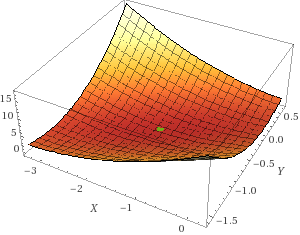
\includegraphics{pic1.png}


	
\end{document}

